\chapter{Multi-node Computation}

\section{Introduction}

In this chapter we describe all base objects (matrices and vectors) for computation on multi-node (distributed-memory) systems. Two typical configurations are presented on Figure \ref{multi-node1} and Figure \ref{multi-node2}.

\begin{figure}[!ht]
\centering
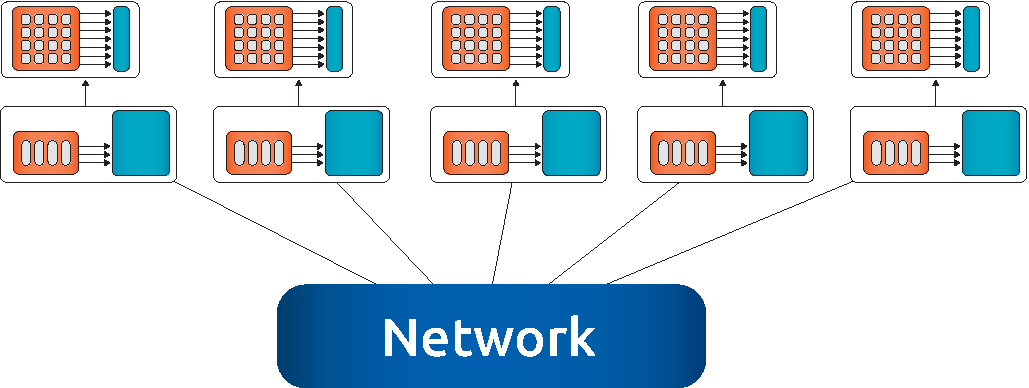
\includegraphics[width=0.6\textwidth]{./fig/multi-node.pdf}
\caption{An example for a multi-node configurations, all nodes are connected via network -- single socket system with a single accelerator.}
\label{multi-node1}
\end{figure}

\begin{figure}[!ht]
\centering
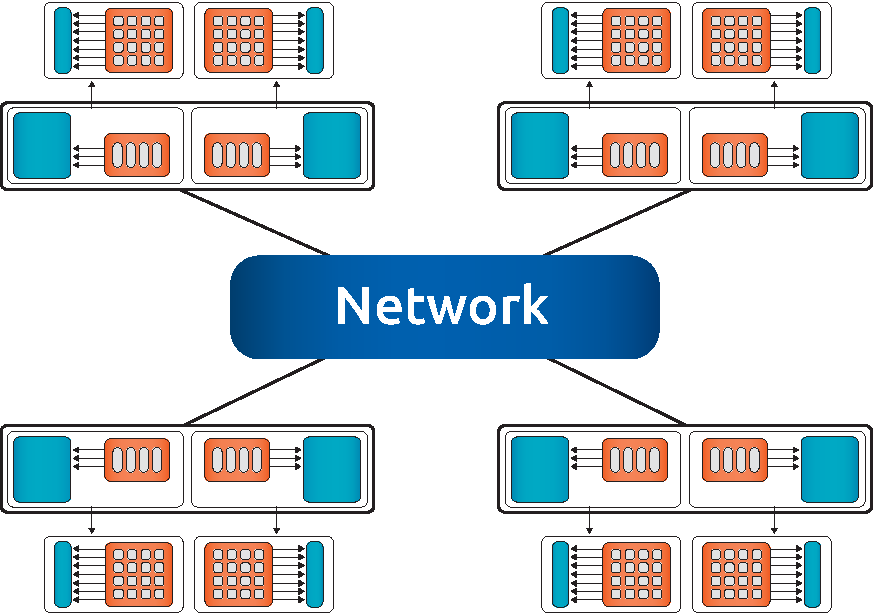
\includegraphics[width=0.6\textwidth]{./fig/multi-node2.pdf}
\caption{An example for a multi-node configurations, all nodes are connected via network -- dual socket systems with two accelerators attached to each node}
\label{multi-node2}
\end{figure}


To each compute node, one or more accelerators can be attached. The compute node could be any kind of shared-memory (single, dual, quad CPU) system, details on a single-node can be found in Figure \ref{single-node}. Note that the memory of the accelerator and of the host are physically different. All nodes can communicate with each other via network.

For the communication channel between the nodes (and between the accelerators on single or multiple nodes) we use the MPI library. Additional libraries for communication can be added on request.

The PARALUTION library supports non-overlapping type of distribution, where the computational domain is split into several sub-domain with the corresponding information about the boundary and ghost layers. An example is shown on Figure \ref{domain-dist}. The square box domain is distributed into four sub-domains. Each subdomain belongs to a process $P0,P1,P2$ and $P3$.

\begin{figure}[!ht]
\centering

\includegraphics[width=0.3\textwidth]{./fig/domain1.pdf}
\hspace{2mm}
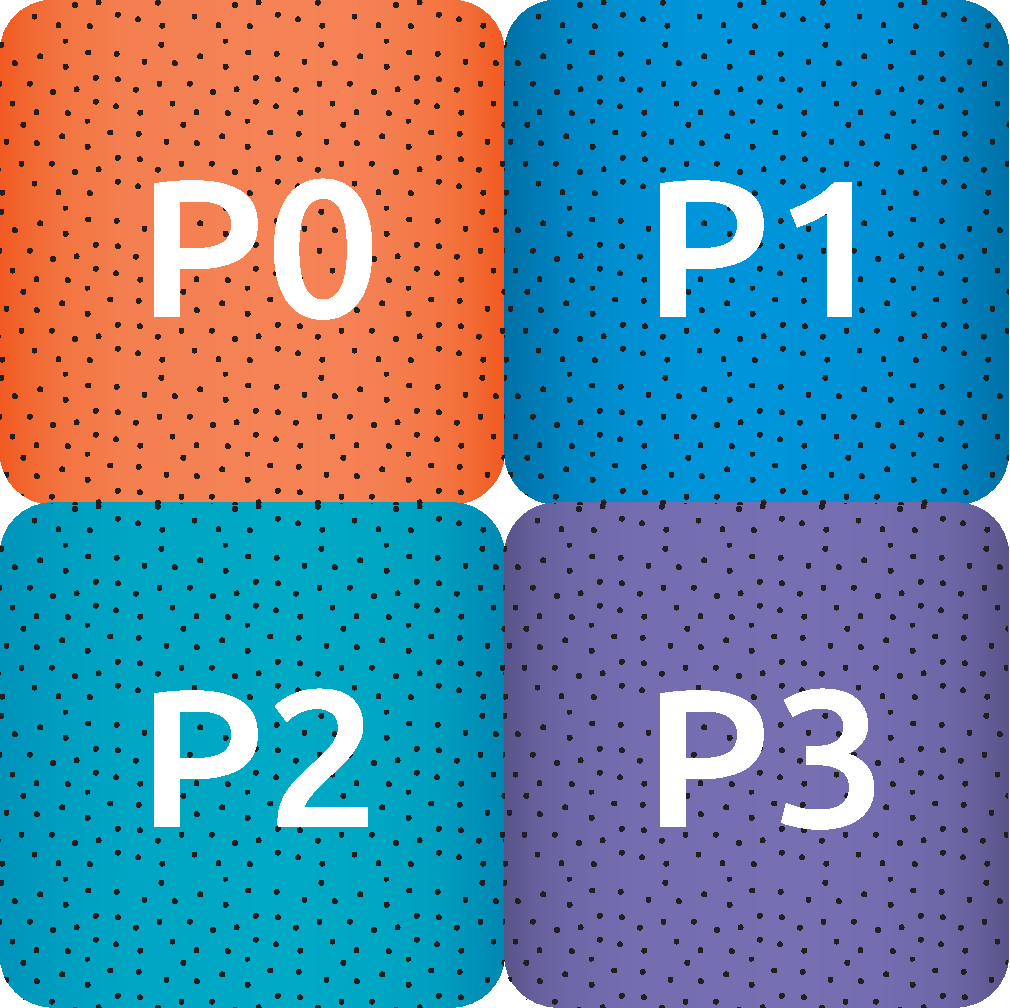
\includegraphics[width=0.3\textwidth]{./fig/domain2.pdf}
\hspace{2mm}
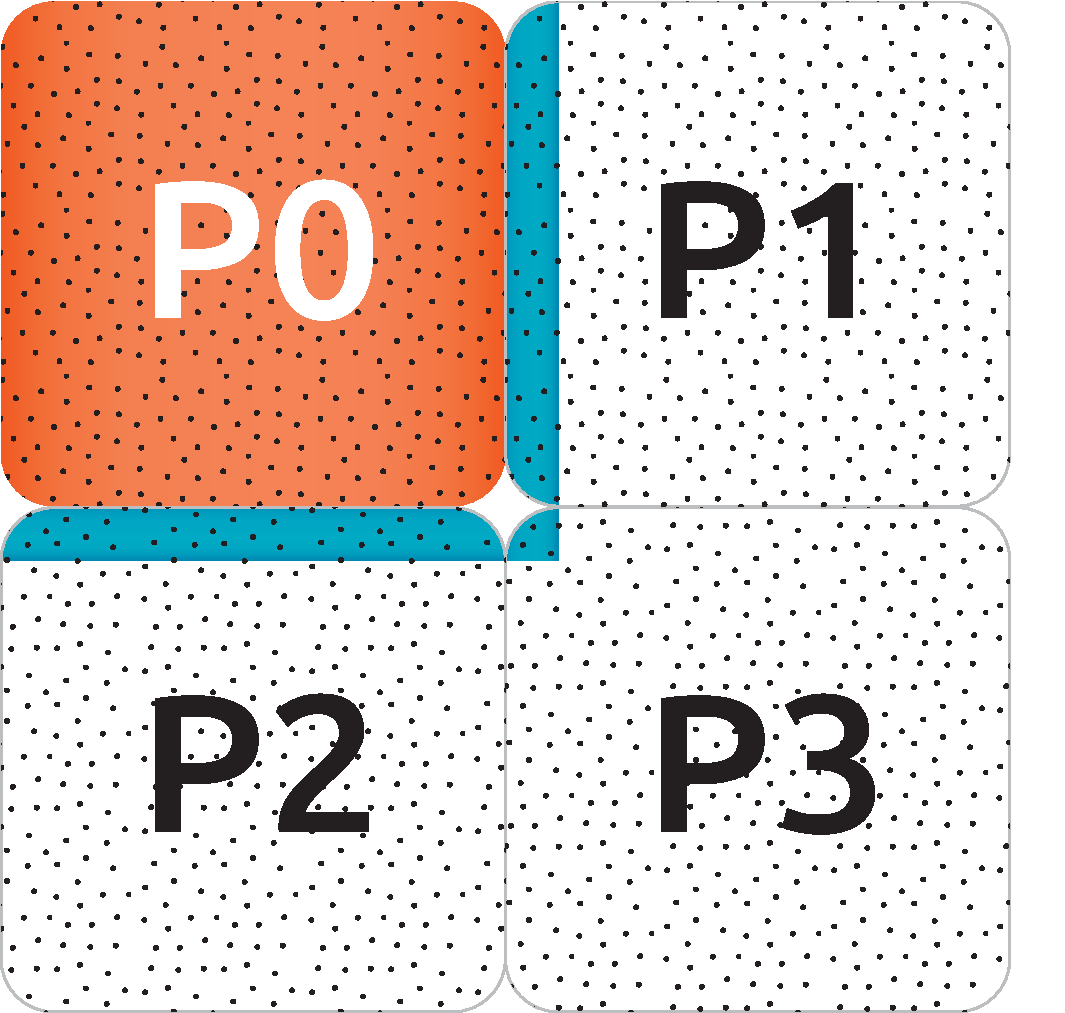
\includegraphics[width=0.3\textwidth]{./fig/domain3.pdf}
\caption{An example for domain distribution}
\label{domain-dist}
\end{figure}

To perform a sparse matrix-vector (SpMV) multiplication, each process need to multiply its own portion of the domain and update the corresponding ghost elements. For $P0$ this multiplication reads
%
\begin{eqnarray}
Ax &=& y, \\
A_{I} x_{I} + A_{G} x_{G} &=& y_{I},
\end{eqnarray}
%
where I stands for interior and G stands for ghost, the $x_{G}$ is a vector with three sections coming from $P1,P2$ and $P3$. The whole ghost part of the global vector is used mainly for the SpMV product and this part of the vector does not play any role in the computation of all vector-vector operations.

\section{Code Structure}

Each object contains two local sub-objects. The global matrix stores the interior and the ghost matrix via local objects. The global vector also stores its data via two local objects. In addition to the local data, the global objects have information about the global communication via the parallel manager  -- see Figure \ref{paralution-global}.

\begin{figure}[!ht]
\centering
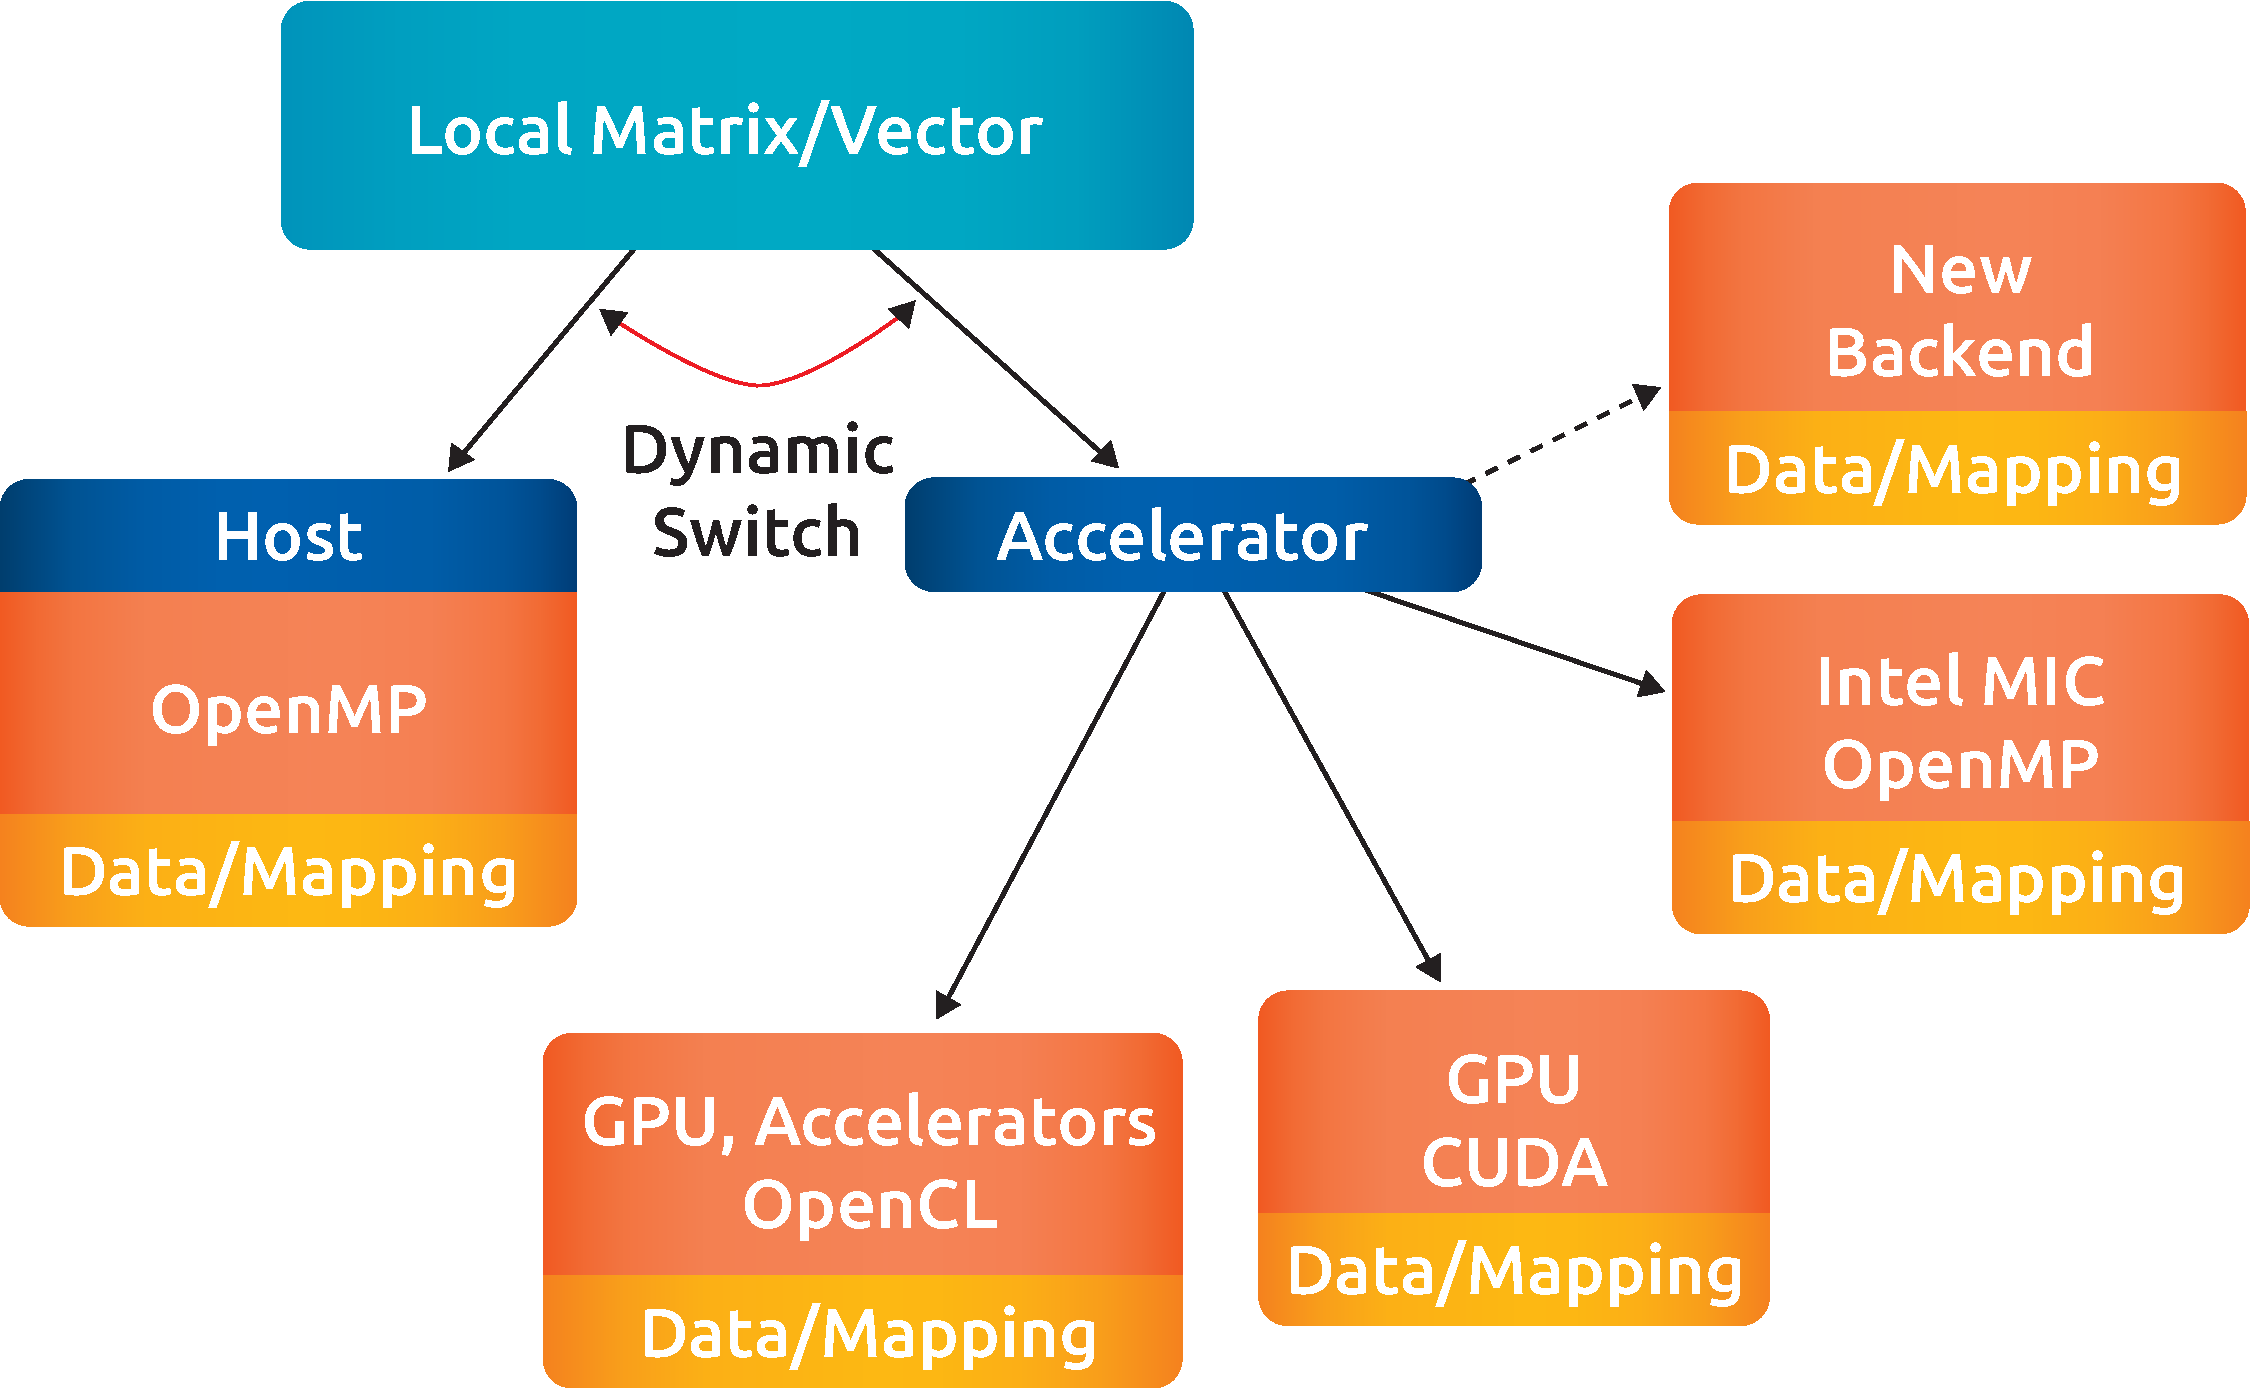
\includegraphics[width=0.6\textwidth]{./fig/global_obj.pdf}
\hspace{7mm}
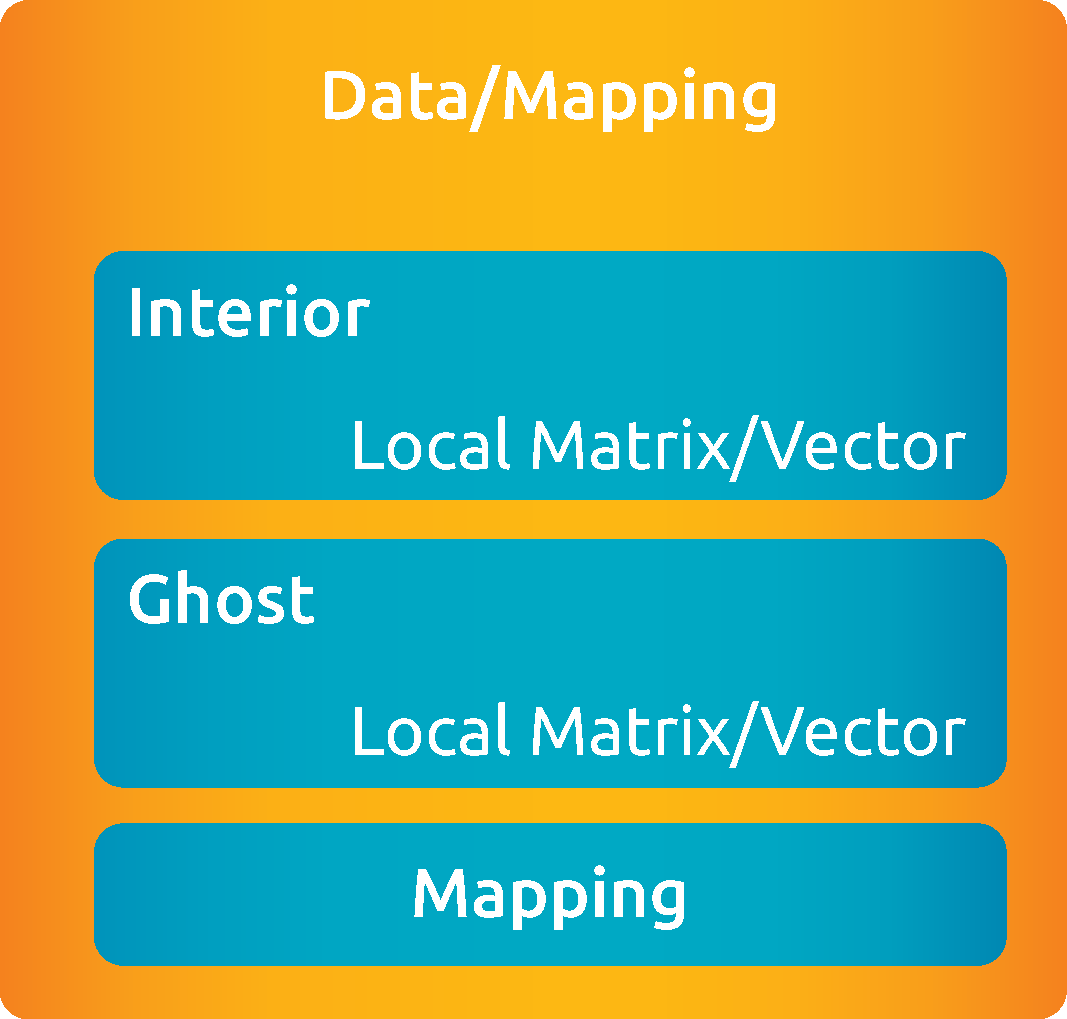
\includegraphics[width=0.3\textwidth]{./fig/global_data.pdf}
\caption{Global Matrices and Vectors}
\label{paralution-global}
\end{figure}

\section{Parallel Manager}

The parallel manager class handles the communication and the mapping of the global matrix. Each global matrix and vector need to be initialized with a valid parallel manager in order to perform any operation.

For many distributed simulation, the underlying matrix is already distributed. This information need to be passed to the parallel manager.

The required information is:
\begin{itemize}
  \item Global size
  \item Local size of the interior/ghost for each rank
  \item Communication pattern (what information need to be sent to whom)
\end{itemize}

\section{Global Matrices and Vectors}

The global matrices and vectors store their data via two local objects. For the global matrix, the interior can be access via the \emph{GetInterior()} and \emph{GetGhost()} functions, which point to two valid local matrices. The same function names exist for the the global vector, which point to two local vector objects.

\subsection{Value Type and Formats}

The value type and the formats can be set in similar manner as in the local matrix. The supported formats are identical to the local case.

\subsection{Matrix and Vector Operations}

Most functions which are available for the local vectors can be performed on the global vector objects as well. For the global matrix, only the SpMV function is supported but all other functions can be performed on the interior of the matrix (without the couplings via the ghost layer).

\subsection{Asynchronous SpMV}

To minimize latency and to increase scalability the PARALUTION library supports asynchronous sparse matrix-vector multiplication. The implementation of the SpMV starts with asynchronous transfer of the needed ghost buffers while at the same time it computes the interior matrix. When the computation of the interior SpMV is done, the ghost transfer is synchronized and the ghost SpMV is performed.

To minimize the PCI-E bus, the OpenCL and CUDA implementation provide a special packaging technique for transferring all ghost data into a contiguous memory buffer.

%\section{Distribution}

\section{Communication Channel}

For the communication channel we use MPI but this can be extended, on request, with some other communication mechanics.

\section{I/O}

The user can store and load the full data from and to files. For a solver, the needed data would be:
\begin{itemize}
  \item Parallel manager
  \item Sparse matrix
  \item Vector 
\end{itemize}

The reading/writing of the data can be done fully in parallel without any communication.

To visualize the data we use $4 \times 4$ grid which is distributed on 4 MPI processes (organized in $2 \times 2$), each local matrix store the local unknowns (with local index) -- see Figure \ref{domain-example}.
\begin{figure}[!ht]
\centering
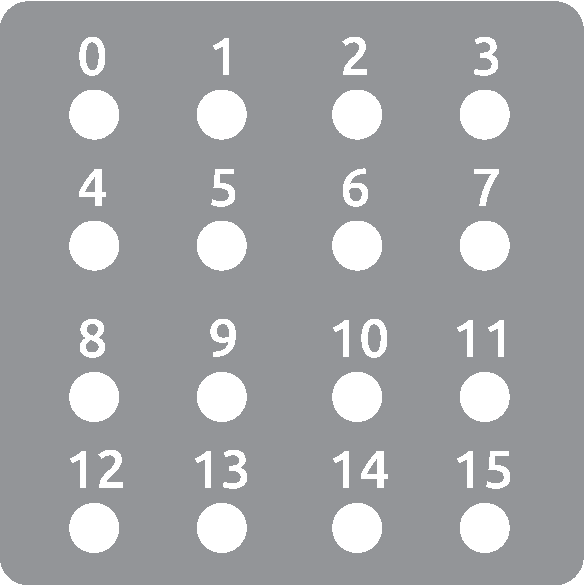
\includegraphics[width=0.2\textwidth]{./fig/mpi-4x4-domain1.pdf}
\hspace{5mm}
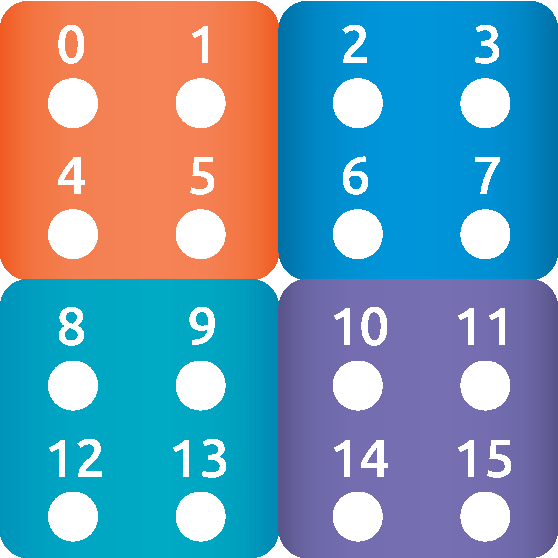
\includegraphics[width=0.2\textwidth]{./fig/mpi-4x4-domain2.pdf}
\caption{An example of $4 \times 4$ grid, distributed in 4 domains ($2 \times 2$)}
\label{domain-example}
\end{figure}

The data associated with RANK 0 is presented on Figure \ref{domain-example-data}.
\begin{figure}[!ht]
\centering
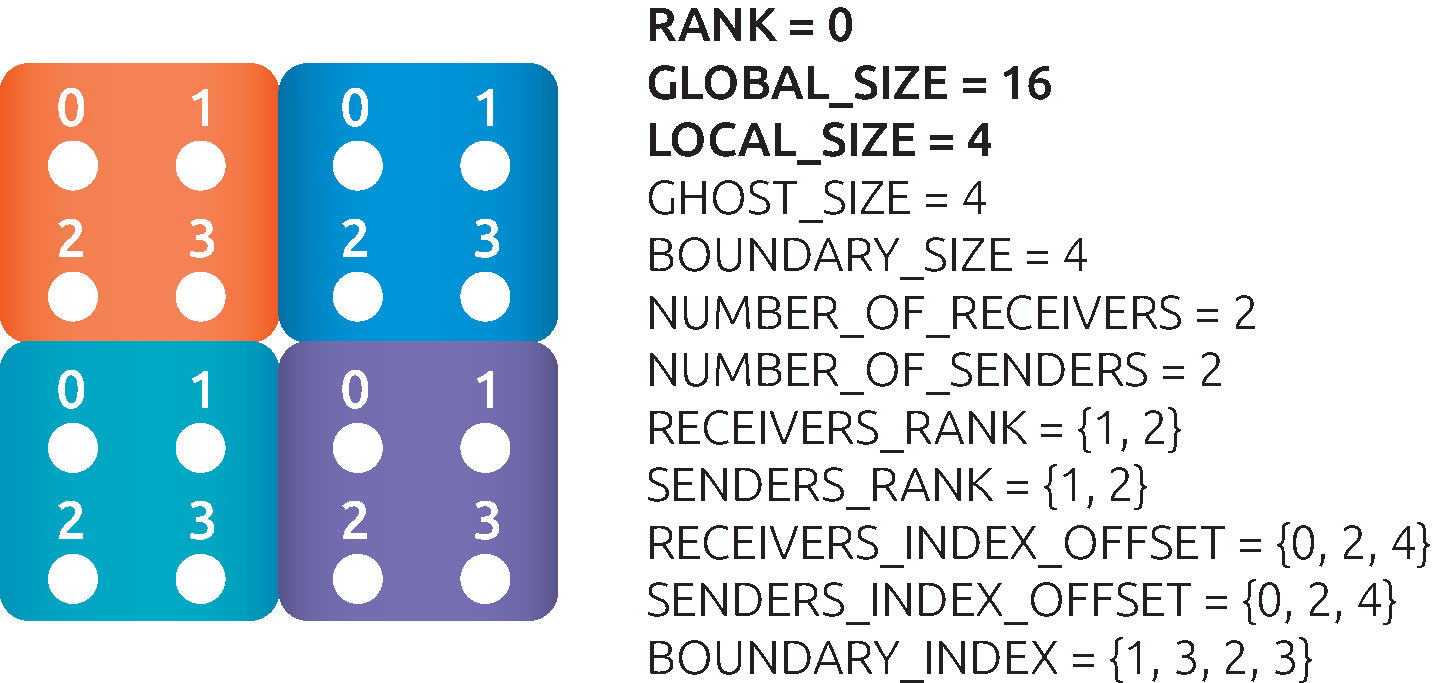
\includegraphics[width=0.6\textwidth]{./fig/mpi-4x4-domain3.pdf}
\caption{An example of 4 MPI process and the data associate with RANK 0}
\label{domain-example-data}
\end{figure}


\subsection{File Organization}

When the parallel manager, global matrix or global vector are writing to a file, the main file (passed as a file name to this function) will contain information for all files on all ranks.

\lstinputlisting[title="Parallel manager (main) file with 4 MPI ranks"]{./src/MPI4/manager.pm}

\lstinputlisting[title="Matrix (main) file with 4 MPI ranks"]{./src/MPI4/matrix.mtx}

\lstinputlisting[title="Vector (main) file with 4 MPI ranks"]{./src/MPI4/rhs.dat}

Example for the data in each file can be found in Section \ref{mpi-laplace-data}.

\subsection{Parallel Manager}

The data for each rank can be seen as two type of information -- one for receiving data from the neighbors, which is presented on Figure \ref{domain-io-rec}. There the RANK0 needs information what type of data will be received, and from whom. The second needed data is the sending information -- RANK0 needs to know where and what to send, see Figure \ref{domain-io-sen}.

\begin{figure}[!ht]
\centering
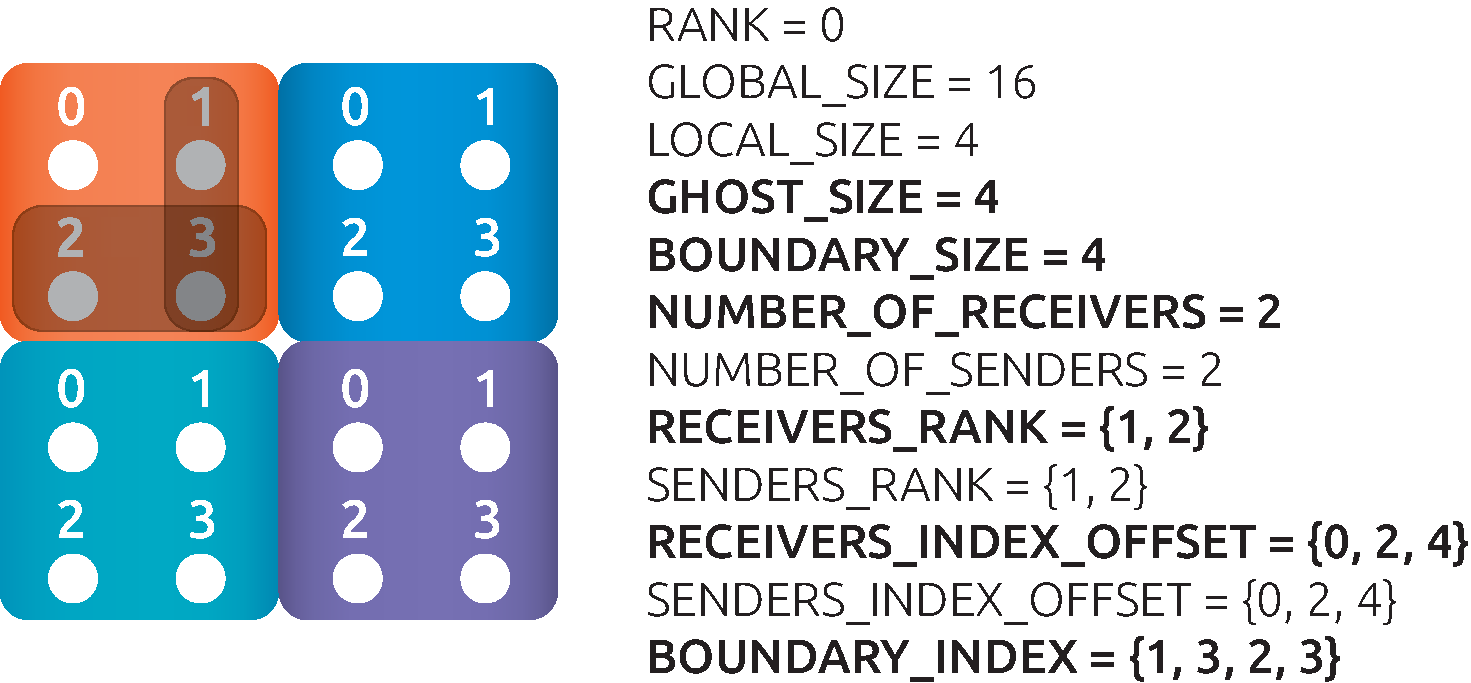
\includegraphics[width=0.6\textwidth]{./fig/mpi-4x4-domain4.pdf}
\caption{An example of 4 MPI process, RANK 0 receives data, the associated data is marked in bold)}
\label{domain-io-rec}
\end{figure}

\emph{Receiving data} -- RANK0 requires:
\begin{itemize}
  \item Total size of the received information (GHOST\_SIZE -- integer value). 
  \item Number of MPI ranks which will send data to RANK0 (NUMBER\_OF\_RECEIVERS -- integer value).
  \item Which are the MPI ranks sending the data (RECEIVERS\_RANK -- integer array).
  \item How the received data (from each rank) will be stored in the ghost vector (RECEIVERS\_INDEX\_OFFSET -- integer array), in this example the first 30 elements will be received from P1 $[0,2)$ and the second 30 from P2 $[2,4)$
\end{itemize}


\begin{figure}[!ht]
\centering
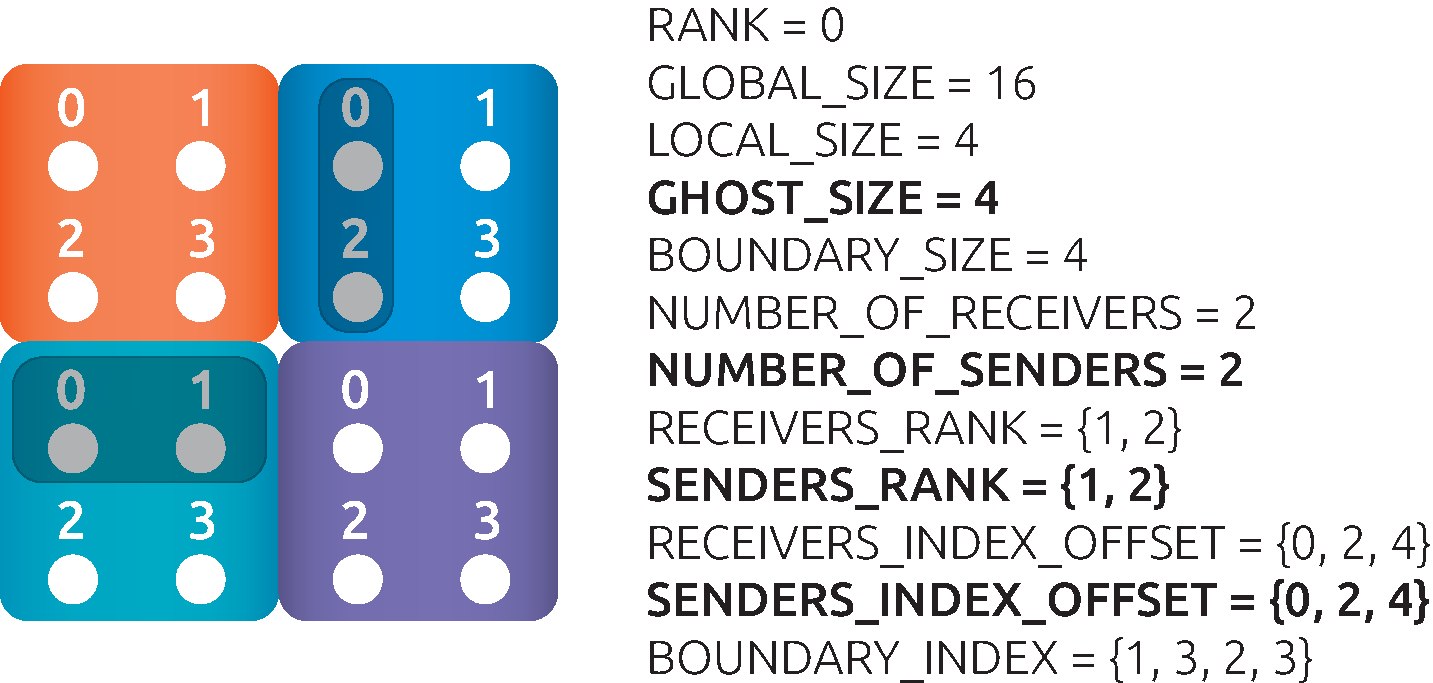
\includegraphics[width=0.6\textwidth]{./fig/mpi-4x4-domain5.pdf}
\caption{An example of 4 MPI process, RANK 0 sends data, the associated data is marked in bold}
\label{domain-io-sen}
\end{figure}

\emph{Sending data} -- RANK0 requires:
\begin{itemize}
  \item Total size of the sending information (BOUNDARY\_SIZE -- integer value). 
  \item Number of MPI ranks which will receive data from RANK0 (NUMBER\_OF\_SENDERS -- integer value).
  \item Which are the MPI ranks receiving the data (SENDERS\_RANK -- integer array).
  \item How the sending data (from each rank) will be stored in the sending buffer (SENDERS\_INDEX\_OFFSET -- integer array), in this example the first 30 elements will be sent to P1 $[0,2)$ and the second 30 to P2 $[2,4)$
  \item The elements which need to be send (BOUNDARY\_INDEX -- integer array). In this example the data which needs to be send to P1 and to P2 is the ghost layer marked as ghost P0. The vertical stripe needs to be send to P1 and the horizontal stripe to P2. The numbering of local unknowns (in local indexing) for P1 (the vertical stripes) are 1, 2 (size of 2) and they are stored in the BOUNDARY\_INDEX. After 2 elements, the elements for P2 are stored, they are 2, 3 (2 elements).
\end{itemize}

\subsection{Matrices}

For each rank, two matrices are used -- interior and ghost matrix. They can be stored in separate files, one for each matrix. The file format could be Matrix Market (MTX) or binary.

\subsection{Vectors}

For each rank, the vector object needs only the local (interior) values. They are stored into a single file. The file could be ASCII or binary.
